\documentclass[letterpaper,11pt]{article}

\usepackage{listings}
\usepackage{color}

\definecolor{dkgreen}{rgb}{0,0.6,0}
\definecolor{gray}{rgb}{0.5,0.5,0.5}
\definecolor{mauve}{rgb}{0.58,0,0.82}

\lstset{frame=tb,
  language=Python,
  aboveskip=3mm,
  belowskip=3mm,
  showstringspaces=false,
  columns=flexible,
  basicstyle={\small\ttfamily},
  numbers=none,
  numberstyle=\tiny\color{gray},
  keywordstyle=\color{blue},
  commentstyle=\color{dkgreen},
  stringstyle=\color{mauve},
  breaklines=true,
  breakatwhitespace=true,
  tabsize=3
}

\usepackage{setspace}
\usepackage{graphicx}
\usepackage{bm}    %for textbf
\usepackage{amsmath}
\usepackage{amsfonts}   %for mathbb
\allowdisplaybreaks[4]  %from {amsmath}
\newcommand{\independent}{\rotatebox[origin=c]{90}{$\models$}}  %from {graphicx}
\usepackage{geometry}
\geometry{letterpaper, scale=0.8}  %from {geometry}
\author{Yuan Yin}
\title{EECS 545 Homework 2}
\begin{document}\large
\maketitle
\begin{spacing}{1.2}  %from {setspace}
\section*{Problem 2}
Code and result is as follows:
\begin{lstlisting}
import numpy as np

# # Process the data
z = np.genfromtxt('spambase.data', dtype = float, delimiter = ',')
np.random.seed(0) # Seed the random number generator
rp = np.random.permutation(z.shape[0]) # random permutation of indices
z = z[rp,:] # shuffle the rows of z
x = z[:,:-1]
y = z[:,-1]

# Quantize variables with option 2 where values equal to the median to 1
row_num,col_num = x.shape; y = list(y)
x_train = x[0:2000,:]
y_train = y[0:2000]
x_test = x[2000:row_num,:]
y_test= y[2000:row_num]

mid_train = np.median(x_train,axis=0)
for i in range(2000):
    for j in range(col_num):
        if x_train[i,j] > mid_train[j]:
            x_train[i,j] = 2
        else:
            x_train[i,j] = 1

# Build up Naive Bayes Classifier
## compute the probability of y=0,1 and the conditional probability of x_j=1,2 given y=0,1
n_1 = sum(y_train); n_0 = len(y_train) - n_1
pi_1 = n_1/len(y_train); pi_0 = 1-pi_1 # the pmf of y
count_x_equ_1_y_equ_0 = np.zeros(col_num)
count_x_equ_1_y_equ_1 = np.zeros(col_num)
count_x_equ_2_y_equ_0 = np.zeros(col_num)
count_x_equ_2_y_equ_1 = np.zeros(col_num)
for l in range(len(y_train)):
    if y_train[l] == 0:
        for m in range(col_num):
            if x_train[l,m] == 1:
                count_x_equ_1_y_equ_0[m] += 1
            elif x_train[l,m] == 2:
                count_x_equ_2_y_equ_0[m] += 1
    elif y_train[l] == 1:
        for n in range(col_num):
            if x_train[l,n] == 1:
                count_x_equ_1_y_equ_1[n] += 1
            elif x_train[l,n] == 2:
                count_x_equ_2_y_equ_1[n] += 1
p_yto0_j_xto1 = np.zeros(col_num)
p_yto1_j_xto1 = np.zeros(col_num)
p_yto0_j_xto2 = np.zeros(col_num)
p_yto1_j_xto2 = np.zeros(col_num)
for i in range(col_num):
    p_yto0_j_xto1[i] = count_x_equ_1_y_equ_0[i]/n_0
    p_yto0_j_xto2[i] = count_x_equ_2_y_equ_0[i]/n_0
for i in range(col_num):
    p_yto1_j_xto1[i] = count_x_equ_1_y_equ_1[i]/(len(y_train)-n_0)
    p_yto1_j_xto2[i] = count_x_equ_2_y_equ_1[i]/(len(y_train)-n_0)

# Test data
## quantize the test data with median of training data, and compute the test result
for i in range(x_test.shape[0]):
    for j in range(x_test.shape[1]):
        if x_test[i,j] > mid_train[j]:
            x_test[i,j] = 2
        else:
            x_test[i,j] = 1

y_test_result = np.zeros(x_test.shape[0])
for i in range(x_test.shape[0]):
    y0 = 1; y1 = 1
    for j in range(x_test.shape[1]):
        if x_test[i,j] == 1:
            y0 = y0*p_yto0_j_xto1[j]
            y1 = y1*p_yto1_j_xto1[j]
        elif x_test[i,j] == 2:
            y0 = y0*p_yto0_j_xto2[j]
            y1 = y1*p_yto1_j_xto2[j]
    if (pi_0*y0) >= (pi_1*y1):
        y_test_result[i] = 0
    else:
        y_test_result[i] = 1

## Test error
error = 0
for i in range(len(y_test)):
    if y_test[i] != y_test_result[i]:
        error += 1
print("The test error of spam emails by Naive Bayes classifier is %f." %(error/len(y_test)) )

## Sanity check
major = 1-y_train.count(1)/len(y_train) # In the training data, the major class for emails is "not spam", so we assume to predict all emails are not spam emails.
error_sanity = y_test.count(1)/len(y_test)
print("The sanity check error is %f." %(error_sanity))
\end{lstlisting}
the result is:
\begin{lstlisting}
The test error of spam emails by Naive Bayes classifier is 0.105344.
The sanity check error is 0.386774.
\end{lstlisting}

\section*{Problem 4}

the code and the result is as follows:
\begin{lstlisting}
from numpy import *
import numpy as np
import scipy.io as sio
import matplotlib.pyplot as plt

# Import the data
mnist_49_3000 = sio.loadmat('mnist_49_3000.mat')
x = mnist_49_3000['x']
y = mnist_49_3000['y']
d,n = x.shape
y += (y < 0) * 1

# Process the data, we divide the data into training part and test part
added = np.ones(n)
x_original = x; y_original = y
x = mat(np.vstack((added,x))); y = mat(y)
x_train = x[:,:2000]; y_train = y[:,:2000]
x_test = x[:,2000:]; y_test= y[:,2000:]

# Initialize parameters
lamda = 10
theta = mat(np.zeros(d + 1))
dJ = mat(np.zeros(d + 1))
d2J = mat(np.zeros([d + 1,d + 1]))

# Iteration with Newton's Method:
## Notice here the stop condition for iteration is when the change of theta is less than 1%
N = 0; error0 = 10
while (error0 > 0.01):
    z = 1 / (1 + np.exp(-theta*x_train))
    dJ = x_train*(z-y_train).T+2*lamda*theta.T
    d2J = x_train * mat(diag(multiply(z, (1-z)).getA()[0])) * x_train.T + 2*lamda*mat(np.eye(d+1,d+1))
    error0 = np.sqrt(((d2J.I * dJ).T * (d2J.I * dJ))[0,0])
    theta = theta - (d2J.I * dJ).T
    y_train_result = theta * x_train
    for l in range(2000):
        if y_train_result[0,l] < 0:
            y_train_result[0,l] = 0
        else:
            y_train_result[0,l] = 1
    N = N+1
print("Iteration times: ", N)
log_like = 0
for l in range(2000):
    z = 1 / (1 + np.exp(-theta * x_train[:,l]))
    log_like += y_train[0,l]*np.log(z)+(1-y_train[0,l])*np.log(1-z)
J = -log_like + lamda*theta*theta.T
print("Value of objective function is: ", J[0,0])

# Test data
y_test_result = theta * x_test
eta_test = 1/(1+np.exp(-y_test_result))
false = []
for l in range(1000):
    if y_test_result[0, l] < 0:
        y_test_result[0, l] = 0
    else:
        y_test_result[0, l] = 1
error1 = 0
for m in range(1000):
    if y_test_result[0, m] != y_test[0, m]:
        error1 += 1
        false.append(m)
print("Test error is: ", error1/1000)
prob = np.zeros(1000)
x_false = x_test[1:,false]; x_false = x_false.getA()
y_false = y_test[:,false]
y_false_result = y_test_result[:,false]
for l in range(1000):
    if y_test_result[0,l] == 0:
        prob[l] = 1-eta_test[0,l]
    else:
        prob[l] = eta_test[0,l]
confidence = prob[false]
indx = argsort(confidence)[28:]
x_false20 = np.zeros((d,20)); y_real20 = np.zeros(20); y_pre20 = np.zeros(20)
for l in range(20):
    x_false20[:,l] = x_false[:,int(indx[l])]
    y_real20[l] = y_false[:,int(indx[l])]
    y_pre20[l] = y_false_result[:,int(indx[l])]

## Plot the picture of 20 most confident missclassified pictures
fig =  plt.figure(num='missclassified',figsize=(8,8))
fig.suptitle("\"True\" represents real result, \"Pre\" represents predicted result\n")
for l in range(20):
    plt.subplot(4,5,1+l)
    if y_real20[l] == 0:
        true_title = 4
        pre_title = 9
    else:
        true_title = 9
        pre_title = 4
    plt.title('True: %s, Pre: %s' %(str(true_title), str(pre_title)))
    plt.imshow(np.reshape(x_false20[:,l], (int(np.sqrt(d)), int(np.sqrt(d)))))
plt.show()
plt.close()
\end{lstlisting}
the result is:

\begin{lstlisting}
Iteration times:  6
Value of objective function is:  307.65546352880267
Test error is:  0.048
\end{lstlisting}

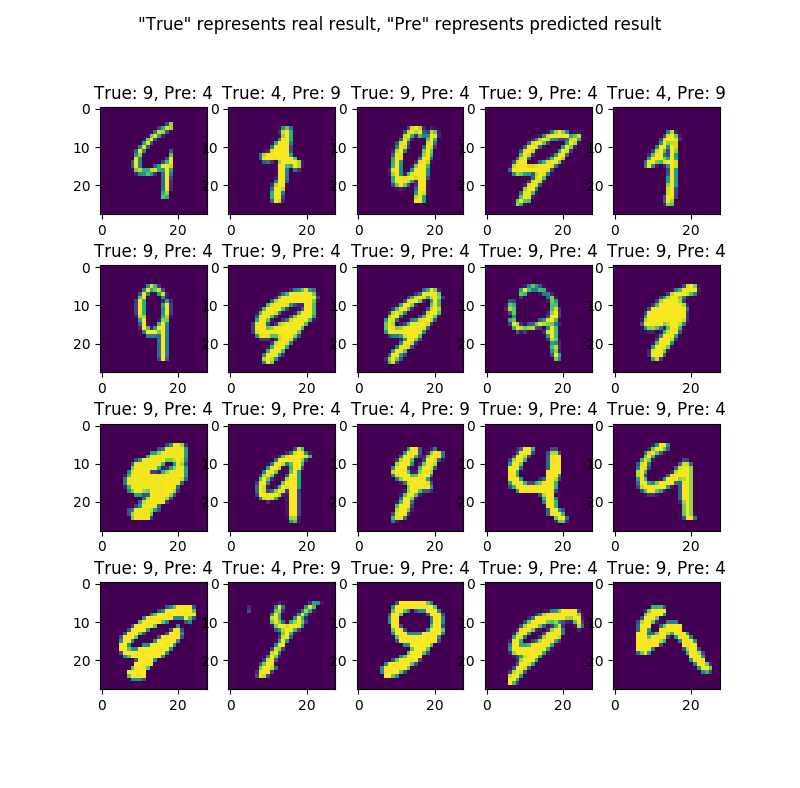
\includegraphics[width=4.72in,height=4.72in]{missclassified.png}

\end{spacing}
\end{document}